\chapter{Conclusions and Future Work}
\label{chap:conclusions}
%Validating my system with an exploratory study is only the first step in a larger design philosophy. I will indicate avenues of improvement for hardware and software focusing on moving to a system on a chip (SoC) design. I will present my conclusions and suggest future steps in the research.

%What Else? form fit issues
% what did the dissertation provide as a fundamental benifit?
% what else should be done, such as shrink all electrodes down to a physical patch.
%look more into spo2 Reflective designs.
\begin{figure}
\centering
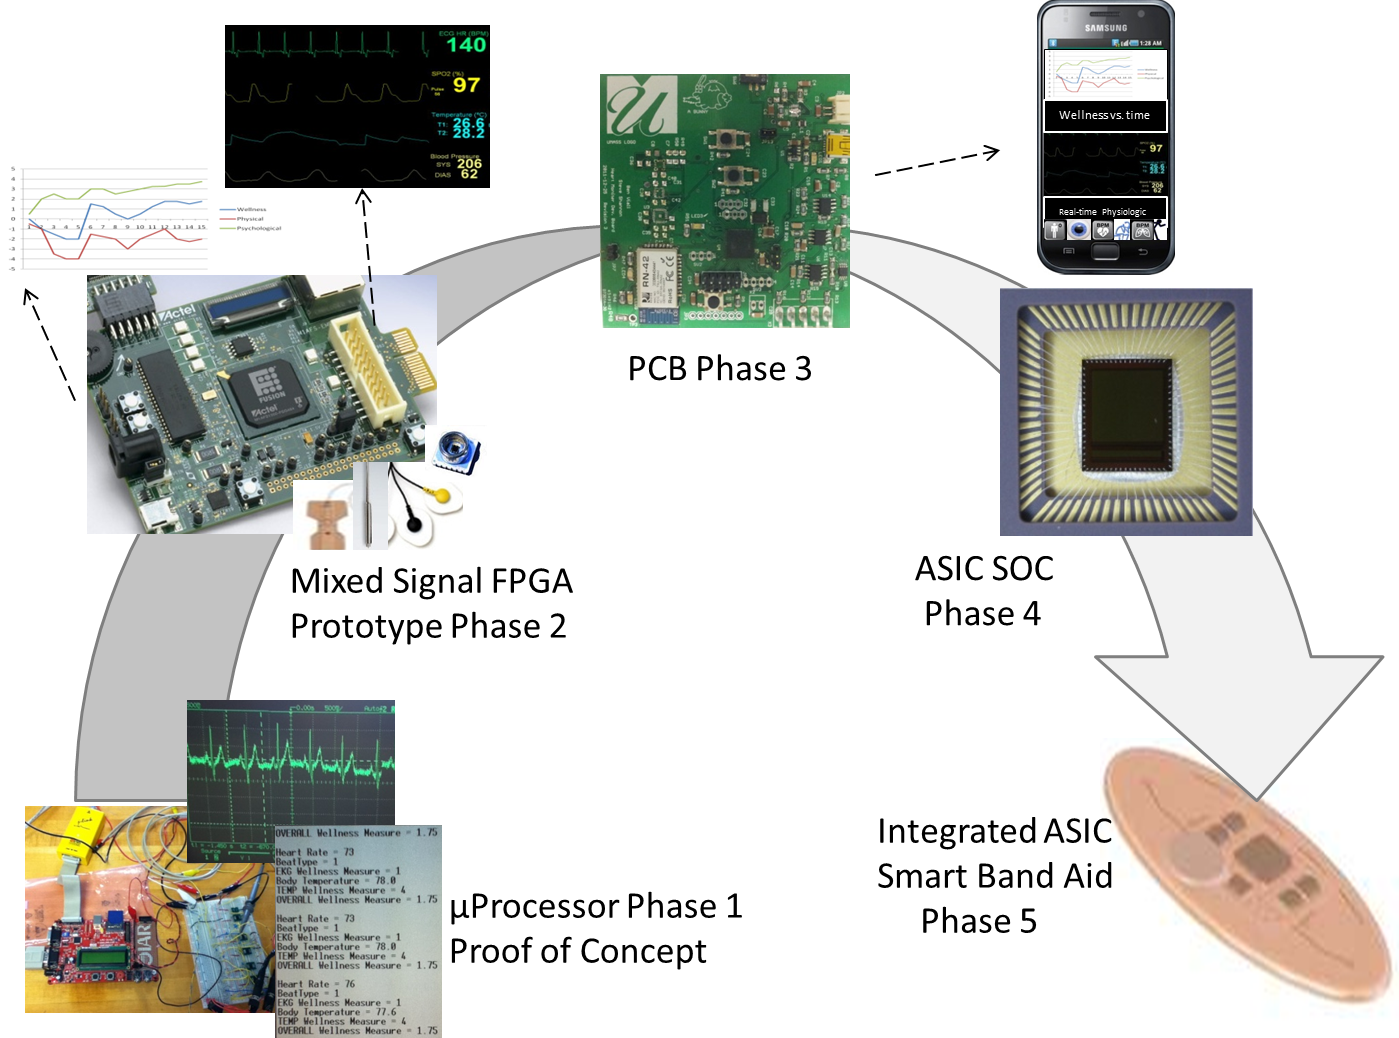
\includegraphics[width=0.7\linewidth]{Images/projectPhases}
\caption{Project Phases}
\label{fig:projectPhases}
\end{figure}


Throughout the process of this dissertation research new findings were always being rolled into the existing framework. The hardware platform for the WHIP sensor was developed from January to May 2014 . This design acquitted itself well through the entire process of the following trial. While some of its functions were under utilized (i.e. the Bluetooth communications) the platform demonstrates an ability to serve as a platform for future research with the ability to support more accurate ECG readings, different \spo2 measuring devices such as nasal alar sensors, and as demonstrated good low power design capabilities. 

A major limitation in the adoption of such a device is a physical constraint not a technological one. The device may be split into smaller modules in future iterations, to more closely contour the human body. This will not be a change to the design of the device, merely a dividing of the modules into different physical PCBs. One approach to increasing adoption of a WHIPPED-like system is to reduce its overall size. Given the work in miniaturizing the various analog front ends\cite{AFE4490,ADS1293}, this design could be miniaturized with appropriate manufacturing support to a disposable patch as proposed in \cref{fig:projectPhases}. The miniaturization of the WHIP sensor would necessitate some fundamental changes in the system design. Foremost, the \spo2 sensor would need to be switched from a transmittance sensor to a reflective sensor. Some preliminary work was done, investigating the integration of a reflective sensor into the design but was abandoned due to time. The sample sensor prototype was designed from the ground up , designed to be as flat as possible. A sensor such as the one shown in  \cref{fig:ReflectiveSensorPrototypes} would then need to be integrated into the sensor strap, or sensor patch.

\begin{figure}
\centering
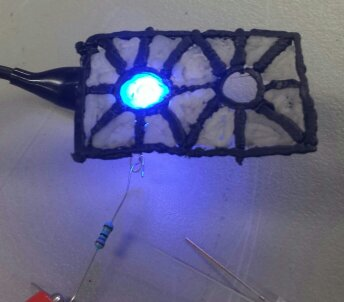
\includegraphics[width=0.5\linewidth]{Images/ReflectiveSensorPrototype.png}
\caption{Reflective Sensor Prototype }
\label{fig:ReflectiveSensorPrototypes}
\end{figure}


The Cellphone was effective at conveying somatic surveys to patients and allowing them to upload information. Future work may include studies on effective user interface choices to simplify the process for patients unfamiliar with cellphone technologies. One problem with the current cell phone approach is updating the surveys during studies, improving the smartphones ability to procure data from a centralized source will make survey maintenance easier in future studies.

In this dissertation, a new sensor platform was developed and tested on a representative heart failure population. The WHIPPED system has been validated as a data gathering tool. The smartphone application has seen continued usage in other studies. The WHIP sensor has shown promise as a platform for longterm data collection. The exploratory trial gave new insights into the potential for the WHIPPED end-to-end system by collecting feedback from patients that can be worked into future iterations of WHIPPED.

